\documentclass[a4paper,10pt]{article}
\usepackage{listings}
\usepackage{color}
\usepackage{algorithm2e}
\usepackage{graphicx}
\usepackage{epstopdf}
\usepackage[margin=1.0in]{geometry}
\usepackage{amsmath,amsthm,amssymb}
 
\definecolor{dkgreen}{rgb}{0,0.6,0}
\definecolor{gray}{rgb}{0.5,0.5,0.5}
\definecolor{mauve}{rgb}{0.58,0,0.82}
 
\lstset{ %
  language=C++,                % the language of the code
  basicstyle=\footnotesize,           % the size of the fonts that are used for the code
  numbers=left,                   % where to put the line-numbers
  numberstyle=\tiny\color{gray},  % the style that is used for the line-numbers
  stepnumber=1,                   % the step between two line-numbers. If it's 1, each line 
                                  % will be numbered
  numbersep=5pt,                  % how far the line-numbers are from the code
  backgroundcolor=\color{white},      % choose the background color. You must add \usepackage{color}
  showspaces=false,               % show spaces adding particular underscores
  showstringspaces=false,         % underline spaces within strings
  showtabs=false,                 % show tabs within strings adding particular underscores
  frame=single,                   % adds a frame around the code
  rulecolor=\color{black},        % if not set, the frame-color may be changed on line-breaks within not-black text (e.g. commens (green here))
  tabsize=2,                      % sets default tabsize to 2 spaces
  captionpos=b,                   % sets the caption-position to bottom
  breaklines=true,                % sets automatic line breaking
  breakatwhitespace=false,        % sets if automatic breaks should only happen at whitespace
  title=\lstname,                   % show the filename of files included with \lstinputlisting;
                                  % also try caption instead of title
  keywordstyle=\color{blue},          % keyword style
  commentstyle=\color{dkgreen},       % comment style
  stringstyle=\color{mauve},         % string literal style
  escapeinside={\%*}{*)},            % if you want to add LaTeX within your code
  morekeywords={*,...}               % if you want to add more keywords to the set
}

% Title Page
\title{Assignment 2: Dynamic Programming project}
\author{Francis Vo, Soo-Hyun Yoo}

\setlength{\parindent}{1cm}
\setlength{\parskip}{1em}

\begin{document}
	\maketitle

	\section{Recursive function}
		\lstinputlisting[language=C++]{rec.cpp}

		\noindent Where {\tt maxS} is a struct holding the running sum and the overall maximum sum and {\tt MaxSubarray} is the recursive function. For an array $A$ of size $n$, we find the maximum subarray with {\tt MaxSubarray(A, n)}.


	\section{Pseudocode}
		\begin{verbatim}
		    MaxSubarray(array, size):
		        current = 0;
		        max = 0;

		        for i=0 to size:
		            current = current + array[i]
		            if current < 0:
		                current = 0
		            else if current > max:
		                max = current

		        return max
		\end{verbatim}


	\section{Running time}
		% Using the Log-Log plot will give us a good hint for the asymptotic run times.  
		% The slope for the graph is 0.987956, meaning that the asymptotic run times is around $\Omega(n)$. 
		% Then looking at the code, it only looks at each element once, making it $\Omega(n)$

		The code shows that we look at each element of the input array only once, so the algorithm's runtime should be $\Theta(n)$.

		Figure~\ref{fig:alg4} shows the execution time of this algorithm versus the size of the input array. The slope of the graph is $0.987956$, which confirms the runtime of $\Theta(n)$.

		\begin{figure}[!htb]
			\centering
			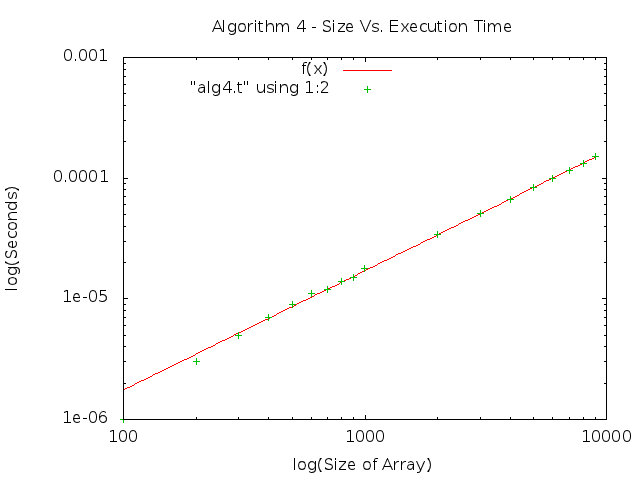
\includegraphics[scale=.5]{timingfiles/alg4plotlog.png}
			\label{fig:alg4}
			\caption{Algorithm 4 -- execution time vs. input size}
		\end{figure}

\begin{samepage} 
	\section{Theoretical correctness}
		\begin{proof}[Induction Proof]
			$MS(k)$ will return the maximum subarray sum for the array $A[0:k]$\\
			\textbf{Base case:} If $n = -1$ then $max = current = 0$\\
			\textbf{Inductive Step:} $maxSubarray(n-1).current + A[n]$ or 0 is the current largest sum starting from the left\\
			\textbf{Proof:}\\ 
			Case if $A[n] > 0$ then $current = MS(n-1).current + A[n] > MS(n-1).current$. \\
			\indent This number might also be the max value. So $max = Greater(max,current)$\\
			Case if $A[n] >  - maxSubarray(n-1)$ then $maxSubarray(n-1) + A[n] < 0$ making the Null set greater.\\
			\indent $max = MS(n-1).max$ and $current = 0$ \\
			Case else making $A[n]$ negative but $maxSubarray(n-1) + A[n] >= 0$\\
			\indent so it is still good to use for the next current: $current + A[n+1] > A[n+1]$\\
			\indent $max = MS(n-1).max$ and $current = maxSubarray(n-1) + A[n]$\\
			$MS(n).max = max$ and $MS(n).current = current$
			 
		\end{proof}
\end{samepage} 
	\section{Implement}
		\subsection{Algorithm 4}
		\lstinputlisting[language=C++]{alg4.cpp}
	\section{Test}
		Test were run on the ms\_test.txt file given last project and large arrays given by student ids.
\begin{samepage} 
	\section{Compare}
		Well, there is a huge difference as seen on the Compare Plot.
		Algorithm 4, Dynamic Programming, is great because doesn't use any recurvsive calls and doesn't need to hold much data.
		Algorithm 4 only needs to hold onto 2 integers (max and current) and the input integer array.  
		Whereas algorithm 3, divide \& conquer, needs to use memory on the stack for each recurvsive call and needs to pass 4 integers back to the parent function.\\
		***WHAT THE HELL IS GOOD ABOUT D\&C???***
		\begin{figure}[!htb]
			\centering
			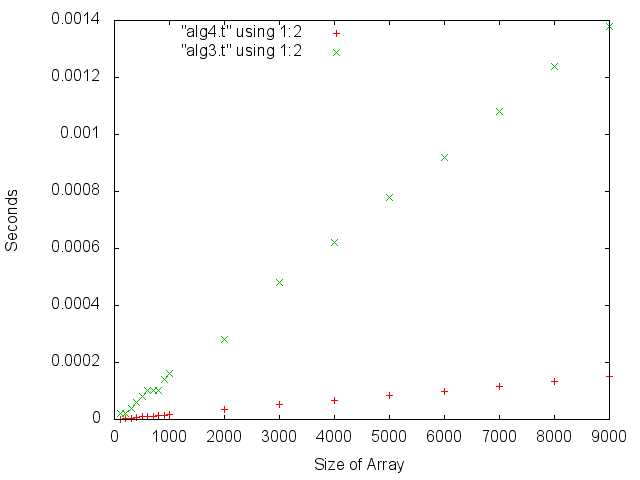
\includegraphics[scale=.5]{timingfiles/algCompareplot.png}
		\end{figure}
\end{samepage} 

		
		

\end{document}
